\documentclass{article}
\usepackage[utf8]{inputenc}
\usepackage{amsmath}
\usepackage{amsfonts}
\usepackage{amssymb}
\usepackage{amsthm}
\usepackage{mathrsfs}
\usepackage{mathtools}
\usepackage{fancyvrb}
\usepackage[margin=1in]{geometry}
\usepackage{fancyhdr}
\usepackage[super]{nth}
\usepackage[T1]{fontenc}
\usepackage{lmodern}
\usepackage{mathrsfs}
\usepackage{tzplot}
\usepackage{pgfplots, tikz}
\newtheorem{theorem}{Theorem}[section]
\newtheorem{lemma}[theorem]{Lemma}
\usepackage{titlesec}
\usepackage{lmodern}
\usepackage{etoolbox}
\usepackage{csquotes}
\usepackage{xcolor}
\usepackage{graphicx}
\usepackage[shortlabels]{enumitem}
\usepackage{listings}
%\usepackage{lipsum}

\makeatletter
\patchcmd{\section}{-3.5ex \@plus -1ex \@minus -.2ex}{-3.5ex \@plus -1ex \@minus -.2ex\setlength{\leftskip}{0cm}}{}{}
\patchcmd{\subsection}{-3.25ex\@plus -1ex \@minus -.2ex}{3.25ex\@plus -1ex \@minus -.2ex\setlength{\leftskip}{0cm}}{}{}
\patchcmd{\subsection}{1.5ex \@plus .2ex}{1.5ex \@plus .2ex\setlength{\leftskip}{2cm}}{}{}
\makeatother
\titleformat{\section}
  {\normalfont\fontsize{12}{15}\bfseries}{\thesection}{1em}{}
\pagestyle{fancy}
\fancyhf{}
\rhead{Aukkawut Ammartayakun}
\lhead{CS 539 Machine Learning: Homework 2}
\cfoot{\thepage}
\title{Homework 2}
\author{Aukkawut Ammartayakun\\CS 539 Machine Learning}
\date{Spring 2023}
\newcommand{\vtt}[1]{%
  \text{\normalfont\ttfamily\detokenize{#1}}%
}



\newcommand{\indep}{\perp \!\!\! \perp}
\begin{document}
\newcommand{\fakesection}[1]{%
  \par\refstepcounter{section}% Increase section counter
  \sectionmark{#1}% Add section mark (header)
  \addcontentsline{toc}{section}{\protect\numberline{\thesection}#1}% Add section to ToC
  % Add more content here, if needed.
}
\newcommand{\fakesubsection}[1]{%
  \par\refstepcounter{subsection}% Increase subsection counter
  \subsectionmark{#1}% Add subsection mark (header)
  \addcontentsline{toc}{subsection}{\protect\numberline{\thesubsection}#1}% Add subsection to ToC
  % Add more content here, if needed.
}
\theoremstyle{definition}
\newtheorem*{sol}{Solution}
\maketitle
\fakesection{q1}
\noindent
\Large{\textbf{Problem 1}}\normalsize
\\

Consider a data set in which each data point $t_n$ is associated with a weighting factor $r_n > 0$, so 
that the sum-of-squares error function becomes  
\begin{equation}
    E_D(\mathbf{w}) = \frac{1}{2}\sum_{n=1}^N r_n\left(t_n - \mathbf{w}^\top\phi(\mathbf{x}_n)\right)^2
\end{equation}
Find  an  expression  for  the  solution  $\mathbf{w}^*$   that  minimizes  this  error  function.  Give  two  alternative 
interpretations of the weighted sum-of-squares error function in terms of (i) data dependent noise variance 
and (ii) replicated data points 

\color{blue}
\begin{sol}
    To minimize the error function, we take the derivative with respect to $\mathbf{w}$.
    \begin{align*}
        \frac{\partial}{\partial \mathbf{w}}E_D(\mathbf{w}) &= -\sum_{n=1}^N r_n\left(t_n - \mathbf{w}^\top\phi(\mathbf{x}_n)\right)\phi(\mathbf{x}_n)
    \end{align*}
    Setting the derivative to zero, we get
    \begin{align*}
        \sum_{n=1}^N r_n\left(t_n - \mathbf{w}^\top\phi(\mathbf{x}_n)\right)\phi(\mathbf{x}_n) &= 0\\
        \sum_{n=1}^N r_n\phi(\mathbf{x}_n)\phi(\mathbf{x}_n)^\top\mathbf{w} &= \sum_{n=1}^N r_n\phi(\mathbf{x}_n)t_n\\
        \mathbf{w} &= \left(\sum_{n=1}^N r_n\phi(\mathbf{x}_n)\phi(\mathbf{x}_n)^\top\right)^{-1}\sum_{n=1}^N r_n\phi(\mathbf{x}_n)t_n
    \end{align*}
\end{sol}
\color{black}
\leavevmode\\
\newpage
\fakesection{q2}
\noindent
\Large{\textbf{Problem 2}}\normalsize
\\

We showed in the class that the conjugate prior for a Gaussian distribution with unknown mean 
and unknown precision (inverse variance) is a normal-gamma distribution. This property also holds for the 
case of the conditional Gaussian distribution $p(t|x,w,\beta)$ of the linear regression model. If we consider the 
likelihood function (3.10), 
\begin{equation}
    p(\mathbf{t}|\mathbf{X},\mathbf{w},\beta) = \prod_{n=1}^N \mathcal{N}(t_n|\mathbf{w}^\top\phi(\mathbf{x}_n),\beta^{-1})
\end{equation}
then the conjugate prior for $\mathbf{w}$ and $\beta$ is given by 
\begin{equation}
    p(\mathbf{w}, \beta) = \mathcal{N}(\mathbf{w}|\mathbf{m}_0,\beta^{-1} \mathbf{S}_0)\text{Gamma}(\beta|a_0,b_0)
\end{equation}
Show that the corresponding posterior distribution takes the same functional form, so that 
\begin{equation}
    p(\mathbf{w}, \beta|\mathbf{t}) = \mathcal{N}(\mathbf{w}|\mathbf{m}_N,\beta^{-1} \mathbf{S}_N)\text{Gamma}(\beta|a_N,b_N)
\end{equation}
and find expressions for the posterior parameters $\mathbf{m}_N$, $\mathbf{S}_N$, $a_N$, and $b_N$. 
\color{blue}
\begin{sol}
    We already know that the conjugate prior is given by
    \begin{align*}
        p(\mathbf{w}, \beta) &= \frac{\sqrt{\beta}}{\sqrt{2\pi}|\mathbf{S}_0|}\exp\left(-\frac{1}{2}\beta(\mathbf{w}-\mathbf{m}_0)^\top S_0^{-1}(\mathbf{w}-\mathbf{m}_0)\right)\frac{\beta^{a_0-1}}{\Gamma(a_0)}b_0^{a_0}\exp(-b_0\beta)
    \end{align*}
    And with the relationship that $\text{posterior} \propto \text{likelihood} \times \text{prior}$, it is clear that the family of the posterior distribution would be Gaussian-gamma distribution. However, the format might be different.
    Now, we want to show that for some constant $k$, 
    \begin{align*}
        kp(\mathbf{t}|\mathbf{w},\beta)p(\mathbf{w}, \beta) = p(\mathbf{w}, \beta|\mathbf{t})
    \end{align*}
    What left is to evaluate the likelihood which is given by
    \begin{align*}
        p(\mathbf{t}|\mathbf{w},\beta) &= \prod_{n=1}^N \mathcal{N}(t_n|\mathbf{w}^\top\phi(\mathbf{x}_n),\beta^{-1})\\
        &= \prod_{n=1}^N \frac{1}{\sqrt{2\pi\beta^{-1}}}\exp\left(-\frac{1}{2}\beta\left(t_n - \mathbf{w}^\top\phi(\mathbf{x}_n)\right)^2\right)
    \end{align*}
    Now, we can evaluate the posterior distribution,
    \begin{align*}
        p(\mathbf{w}, \beta|\mathbf{t}) &= k\frac{\sqrt{\beta}}{\sqrt{2\pi}|\mathbf{S}_0|}\exp\left(-\frac{1}{2}\beta(\mathbf{w}-\mathbf{m}_0)^\top \mathbf{S}_0^{-1}(\mathbf{w}-\mathbf{m}_0)\right)\frac{\beta^{a_0-1}}{\Gamma(a_0)}b_0^{a_0}\exp(-b_0\beta) \prod_{n=1}^N \frac{1}{\sqrt{2\pi\beta^{-1}}}\exp\left(-\frac{1}{2}\beta\left(t_n - \mathbf{w}^\top\phi(\mathbf{x}_n)\right)^2\right)\\
        &= k\frac{b_0^{a_0}\exp(-b_0\beta)\beta^{a_0+N/2-1}}{\Gamma(a_0)\sqrt{2\pi}|\mathbf{S}_0|}\exp\left(-\frac{1}{2}\beta\left[\left(\mathbf{w}-\mathbf{m}_0\right)^\top \mathbf{S}_0^{-1}\left(\mathbf{w}-\mathbf{m}_0\right) +\sum_{n=1}^N\left(t_n - \mathbf{w}^\top\phi(\mathbf{x}_n)\right)^2\right]\right)
    \end{align*}
    it is clear that from the multiplication,
    $\mathbf{S}_N^{-1} = \mathbf{S}_0^{-1} + \sum_{n=1}^N \phi(\mathbf{x}_n)\phi(\mathbf{x}_n)^\top$ and $\mathbf{m}_N = \mathbf{S}_N\left(\mathbf{S}_0^{-1}\mathbf{m}_0 + \sum_{n=1}^N \phi(\mathbf{x}_n)t_n\right)$
    Thus,
    \begin{align*}
        \mathbf{S}_N &= \left(\mathbf{S}_0^{-1} + \sum_{n=1}^N \phi(\mathbf{x}_n)\phi(\mathbf{x}_n)^\top\right)^{-1}\\
        \mathbf{m}_N &= \mathbf{S}_N\left(\mathbf{S}_0^{-1}\mathbf{m}_0 + \sum_{n=1}^N \phi(\mathbf{x}_n)t_n\right)
    \end{align*}
    and for $a_N$ and $b_N$, we have
    \begin{align*}
        a_N &= a_0 + \frac{N}{2}\\
        b_N &= b_0 + \frac{1}{2}\sum_{n=1}^N\left(t_n - \mathbf{w}^\top\phi(\mathbf{x}_n)\right)^2 + \frac{1}{2}\mathbf{m}_0^\top\mathbf{S}_0^{-1}\mathbf{m}_0 - \frac{1}{2}\mathbf{m}_N^\top\mathbf{S}_N^{-1}\mathbf{m}_N
    \end{align*}
\end{sol}
\color{black}
\leavevmode\\
\fakesection{q3}
\noindent
\Large{\textbf{Problem 3}}\normalsize
\\

Show  that  for  a  linearly  separable  data  set,  the  maximum  likelihood  solution  for  the  logistic 
regression model is obtained by finding a vector $\mathbf{w}$ whose decision boundary $\mathbf{w}^\top\phi(\mathbf{x}) = 0$ separates the 
classes and then taking the magnitude of $\mathbf{w}$ to infinity 
\color{blue}
\begin{sol}
   Intuitively, we can see that $\mathbf{w}^\top\phi(\mathbf{x}) \geq 0$ for all $\mathbf{x}$ corresponding to a class $y_i$. Thus, the decision boundary would be $\mathbf{w}^{\top} \phi(\mathbf{x}) = 0$. Looking at the likelihood function of this Bernoulli process,
    \begin{align*}
        p(\mathbf{x}|y_i,\mathbf{w}) &= \prod_{i=1}^{n} \left(\frac{1}{1 + e^{-w^T x_i}}\right)^{y_i} \left(1 - \left(\frac{1}{1 + e^{-w^T x_i}}\right)\right)^{1-y_i}\\
        \ln p(\mathbf{x}|y_i,\mathbf{w}) &= \sum_{i=1}^{n} \left(y_i\ln\left(\frac{1}{1 + e^{-w^T x_i}}\right) + (1-y_i)\ln\left(1 - \left(\frac{1}{1 + e^{-w^T x_i}}\right)\right)\right)
    \end{align*}
    to maximize the log-likelihood here, it is clear that the magnitute of $\mathbf{w}$ should be as large as possible.
\end{sol}
\color{black}
\leavevmode\\
\fakesection{q4}
\noindent
\Large{\textbf{Problem 4}}\normalsize
\\

Show  that  the  Hessian  matrix  $\mathbf{H}$  for  the  logistic  regression  model,  given  by  (4.97),  
\begin{equation}
    \mathbf{H} = \nabla\nabla E(\mathbf{w}) = \sum_{n=1}^N y_n(1-y_n)\mathbf{\phi}_n\mathbf{\phi}_n^\top = \mathbf{\Phi}^{\top} \mathbf{R}\mathbf{\Phi}
\end{equation}
is  positive definite.  Here  $\mathbf{R}$  is  a  diagonal  matrix  with  elements  $y_n(1-y_n)$,  and  $y_n$  is  the  output  of  the  logistic 
regression model for input vector  $\mathbf{x}_n$. Hence show that the error function is a concave function of $\mathbf{w}$ and 
that it has a unique minimum. 
\color{blue}
\begin{sol}
It is clear that $y_n(1-y_n)$ is positive for all $n$. Thus, $\mathbf{R}$ is positive definite. Thus, $\mathbf{H}$ is positive definite.
And as we know, a function is concave if its Hessian is positive definite. Thus, the error function is a concave function of $\mathbf{w}$.
Also, with the concavity, we know that the error function has a unique minimum.
\end{sol}
\color{black}
\leavevmode\\

\fakesection{q5}
\noindent
\Large{\textbf{Problem 5 (Likelihood Estimate for Gamma regression)}}\normalsize
\\

Gamma distribution is defined by  
\begin{equation}
    f(x|\alpha, \beta) = \frac{\beta^\alpha}{\Gamma(\alpha)} x^{\alpha-1} e^{-\beta x}
\end{equation}
\begin{enumerate}
    \item Write down the probability in general form of the exponential distribution family, and find 
    natural parameter $\eta$, $u(x)$, $h(x)$, and $g(\eta)$.
    \color{blue}
    \begin{sol}
        \begin{align*}
            f(x|\alpha,\beta) &= h(x)g(\eta)\exp(\eta^\top u(x))\\
            \eta &= \left[\alpha - 1, -\beta\right]^\top\\
            u(x) &= \left[\ln x, -x\right]^\top\\
            h(x) &= 1\\
            g(\eta) &= \frac{\beta^\alpha}{\Gamma(\alpha)}
        \end{align*}
    \end{sol}
    \color{black}
    \item Let’s assume we have a set of data points $(t_i,x_i)\; i = 1, \dots, N$, and we assume $t_i$ follows a Gamma 
    distribution where its mean is defined by
    \begin{equation}
        y_k = \exp\left(w_0 + w_1 x_k\right)
    \end{equation}
    and the conditional distribution is 
    \begin{equation}
        f(t_k|y_k) =  \frac{1}{\Gamma(\nu)}\left(\frac{\nu t_k}{y_k}\right)^{\nu} \frac{1}{y_k} e^{-\frac{\nu t_k}{y_k}}
    \end{equation}
    discuss how you can find maximum likelihood estimates of $w_0$ and $w_1$ using a gradient ascent algorithm. Derive the gradient and discuss whether the likelihood function is a concave function of the $w_0$ and $w_1$ or not.
    \color{blue}
    \begin{sol}
        We can see that $f(t_k|y_k)$ is a Gamma distribution with parameters $\alpha = \nu$ and $\beta = \nu/y_k$. Thus, we can write down the log-likelihood function as
        Given that Gamma distribution is in the exponential family, we can write down the log-likelihood function as
        \begin{align*}
            p(\mathbf{t}|\mathbf{y}) = \sum_{k=1}^{N} \left(\ln\left(\frac{\nu}{y_k}\right) - \frac{\nu t_k}{y_k} - \ln \Gamma(\nu)\right)
        \end{align*}
        Substituting $y_k = \exp\left(w_0 + w_1 x_k\right)$, we have
        \begin{align*}
            p(\mathbf{t}|\mathbf{y}) &= \sum_{k=1}^{N} \left(\ln\left(\frac{\nu}{\exp\left(w_0 + w_1 x_k\right)}\right) - \frac{\nu t_k}{\exp\left(w_0 + w_1 x_k\right)} - \ln \Gamma(\nu)\right)\\
            &= \sum_{k=1}^N \left(\ln(\nu) - (w_0+w_1 x_k) - \nu t_k \exp(w_0 + w_1x_k) - \ln \Gamma(\nu)\right)
        \end{align*}
        Find the gradient of the log-likelihood function with respect to $w_0$ and $w_1$:
        \begin{align*}
            \frac{\partial p(\mathbf{t}|\mathbf{y})}{\partial w_0} &= -\sum_{k=1}^{N} \left(\nu t_k\exp(w_0 + w_1 x_k) + 1  \right)\\
            \frac{\partial p(\mathbf{t}|\mathbf{y})}{\partial w_1} &= -\sum_{k=1}^{N} \left(\nu t_k x_k \exp(w_0 + w_1 x_k) + x_k\right)
        \end{align*}
        As exponential function is convex, its negative is concave. Thus, the log-likelihood function is concave. That means, we can use the gradient ascent to find the maximum likelihood estimates of $w_0$ and $w_1$.
        This can be done by updating the parameters $w_0$ and $w_1$ as
        \begin{align*}
            w_0 &\leftarrow w_0 + \eta \frac{\partial p(\mathbf{t}|\mathbf{y})}{\partial w_0}\\
            w_1 &\leftarrow w_1 + \eta \frac{\partial p(\mathbf{t}|\mathbf{y})}{\partial w_1}
        \end{align*}
        for some learning rate $\eta$.
    \end{sol}
    \color{black}
\end{enumerate}
\leavevmode\\
\fakesection{q6}
\noindent
\Large{\textbf{Problem 6 (Laplacian Prior)}}\normalsize
\\

Laplacian prior for the weights of a linear (or logistic) regression will turn into 
Lasso regularization. Laplacian distribution on $w$ is defined by 
\begin{equation}
    p(\mathbf{w}) = \frac{1}{2b} \exp\left(-\frac{|\mathbf{w}|}{b}\right)
\end{equation}
which can be defined for weights of the model (except the intercept), where we assume different weigths 
are independent. $b$ is a hyperparameter. 
\begin{enumerate}
    \item Let’s assume we have $D = \{(\mathbf{x}_i,t_i)| i = 1, \dots, N\}$  and  we  want  to  build  a  linear  regression  model 
    with the Laplacian prior on the model weights. Define the likelihood and prior term here, and show it turns 
    to a lasso regression. You can assume weights share the same hyperparameter. 
    \color{blue}
    \begin{sol}
        Let say we have a linear regression model with Laplacian prior on the weights. The likelihood term is
        \begin{equation*}
            p(\mathbf{t}|\mathbf{X},\mathbf{w}) = \prod_{i=1}^N \frac{1}{\sqrt{2\pi\sigma^2}} \exp\left(-\frac{(t_i - \mathbf{w}^\top\phi(\mathbf{x}_i))^2}{2\sigma^2}\right)
        \end{equation*}
        and the prior term is
        \begin{equation*}
            p(\mathbf{w}) = \frac{1}{2b} \exp\left(-\frac{|\mathbf{w}|}{b}\right)
        \end{equation*}
        The posterior distribution is proportional to the likelihood and prior term
        \begin{equation*}
            p(\mathbf{w}|\mathbf{X},\mathbf{t}) \propto p(\mathbf{t}|\mathbf{X},\mathbf{w})p(\mathbf{w})
        \end{equation*}
        or
        \begin{equation*}
            p(\mathbf{w}|\mathbf{X},\mathbf{t}) \propto \prod_{i=1}^N \frac{1}{\sqrt{2\pi\sigma^2}} \exp\left(-\frac{(t_i - \mathbf{w}^\top\phi(\mathbf{x}_i))^2}{2\sigma^2}\right) \frac{1}{2b} \exp\left(-\frac{|\mathbf{w}|}{b}\right)
        \end{equation*}
        MAP estimation would be
        \begin{align*}
            \mathbf{w}^* &= \arg\max_{\mathbf{w}} p(\mathbf{w}|\mathbf{X},\mathbf{t})\\
            &= \arg\max_{\mathbf{w}} \ln p(\mathbf{w}|\mathbf{X},\mathbf{t})\\
            &= \arg\max_{\mathbf{w}} \ln \prod_{i=1}^N \frac{1}{\sqrt{2\pi\sigma^2}} \exp\left(-\frac{(t_i - \mathbf{w}^\top\phi(\mathbf{x}_i))^2}{2\sigma^2}\right) \frac{1}{2b} \exp\left(-\frac{|\mathbf{w}|}{b}\right)\\
            &= \arg\max_{\mathbf{w}} \sum_{i=1}^N \ln \frac{1}{\sqrt{2\pi\sigma^2}} -\frac{(t_i - \mathbf{w}^\top\phi(\mathbf{x}_i))^2}{2\sigma^2} + \ln \frac{1}{2b} -\frac{|\mathbf{w}|}{b}\\
            &= \arg\max_{\mathbf{w}} -\frac{1}{2}\sum_{i=1}^N \frac{(t_i - \mathbf{w}^\top\phi(\mathbf{x}_i))^2}{2\sigma^2} +\frac{2|\mathbf{w}|}{b}
        \end{align*}
        which shows the sum-of-squares error with penalty term in the lasso regression.
        \end{sol}
    \color{black}
    \item Lasso regression is defined by
    \begin{equation}
        E_D(\mathbf{w}) = -\frac{1}{2}\sum_{i=1}^N (t_i - \mathbf{w}^\top\phi(\mathbf{x}_i))^2 - \lambda\sum_{j=1}^M |w_j|
    \end{equation}
    We can use a gradient descent algorithm to find the model parameters, but the issue is that derivative of $|\mathbf{w}|$ has a discontinuity at zero. A remedy is to rewrite the optimization by
    \begin{equation}
        E_D(\mathbf{w}) = -\frac{1}{2}\sum_{i=1}^N (t_i - \mathbf{w}^\top\phi(\mathbf{x}_i))^2 - \lambda\sum_{j=1}^M \frac{w_j^2}{|w_j|}
    \end{equation}
    where, you replace the term in denominator of the regularization term by a known value. Let’s assume, you are in the $r^{\text{th}}$ iteration of a gradient descent algorithm ($r$ represents the iteration), and your partial 
    derivative for $j^{\text{th}}$ weight is defined by 
    \begin{equation}
        \dfrac{\partial E_D^{(r)}(\mathbf{w})}{\partial w_j} \approx \sum_{i=1}^{N} \phi(\mathbf{x}_i)\left(t_i - {\mathbf{w}^{(r)}}^\top \phi(\mathbf{x}_i)\right) - \lambda \frac{w_j^{(r)}}{\max \left\{\epsilon, |w_j^{(r-1)}|\right\}}
    \end{equation}
    where, $\epsilon$ has a small value, like 0.0001. Complete the update rule for all other weights in the model and show its result in a simulated data.  
    \color{blue}
    \begin{sol}
    The update rule for the $j^{\text{th}}$ weight is
    \begin{equation}
        w_j^{(r+1)} = w_j^{(r)} - \eta \left(\sum_{i=1}^{N} \phi(\mathbf{x}_i)\left(t_i - {\mathbf{w}^{(r)}}^\top \phi(\mathbf{x}_i)\right) - \lambda \frac{w_j^{(r)}}{\max \left\{\epsilon, |w_j^{(r-1)}|\right\}}\right)
    \end{equation}
    and the update rule for all other weights is the same.
    The simulation code is given below.
    \begin{lstlisting}
import numpy as np
np.random.seed(0)
N = 100
x = np.random.randn(N, 1)
y = 3 + 2 * x + np.random.randn(N, 1)
phi = x
alpha = 0.01
lambda_ = 0.1
max_iter = 10
w = np.zeros((2, 1))
weights = np.zeros((max_iter, 2))
obj = np.zeros((max_iter, 1))
for r in range(max_iter):
    for i in range(w.size):
        obj[r] = 0.5 * np.sum((y[i] - np.dot(phi[i], w[i])) ** 2) + 
        lambda_ * np.sum((w[i] ** 2)/ np.abs(w[i]))
        grad = -np.dot(phi[i], y[i] - np.dot(phi[i], w[i])) + 
        lambda_ * w[i]/max(np.abs(w[i]), 0.0001)
        w[i] = w[i] - alpha * grad
        weights[r,i] = w[i]
    \end{lstlisting}
    \begin{figure}[!ht]
        \centering
        \begin{tikzpicture}
            \begin{axis}[
            xlabel={Iteration},
            ylabel={Weights},
            legend style={at={(0.5,-0.2)},anchor=north,legend columns=-1}]
            \addplot[blue,mark=none] table[x index=0,y index=1] {weights.txt};
            \addplot[red,mark=none] table[x index=0,y index=0] {weights.txt};
            \legend{$w_1$, $w_0$}
            \end{axis}
            \end{tikzpicture}
    \end{figure}
    \end{sol}
    \color{black}
    
    \item Create 100 sample data points for $t_i = 1 + 0.001 \mathbf{x}_i - 2 \mathbf{x}_i^2 +\epsilon_k$ where $\epsilon_k$ has normal distribution 
    with a mean zero and variance of 0.1. Show how the estimated weights will change as a function of $\lambda$. For 
    $x$, you can draw  100 random values from a normal distribution with mean 0 and variance 1. To find the 
    model parameters you can use the gradient descent algorithm we discussed here. 
    \color{blue}
    \begin{sol}
    The simulation code is given below.
    \begin{lstlisting}
import numpy as np
import matplotlib.pyplot as plt
np.random.seed(0)
N = 1000
x = np.random.randn(N, 1)
epsilon = np.random.randn(N, 1) * np.sqrt(0.1)
t = 1 + 0.001 * x - 2 * x ** 2 + epsilon
phi = np.hstack((np.ones((N, 1)), x, x ** 2))
alpha = 1e-6
lambda_ = np.array([0, 0.1, 1, 10])
max_iter = 100
w = np.zeros((3, 1))
obj = np.zeros((len(lambda_), max_iter))
for i, l in enumerate(lambda_):
    for r in range(max_iter):
        obj[i, r] = 0.5 * np.sum((t - np.dot(phi, w)) ** 2) + 
        l * np.sum(np.abs(w[1:]))
        grad = -np.dot(phi.T, t - np.dot(phi, w)) + 
        l * np.vstack((0, l * np.sign(w[1:])))
        w = w - alpha * grad
for i in range(len(lambda_)):
    plt.plot(range(max_iter), obj[i, :], label='lambda = {:.3f}'.format(lambda_[i]))
plt.xlabel('Iteration')
plt.ylabel('Objective Function')
plt.legend()
plt.show()

    \end{lstlisting}
    \begin{figure}[!ht]
        \begin{center}
        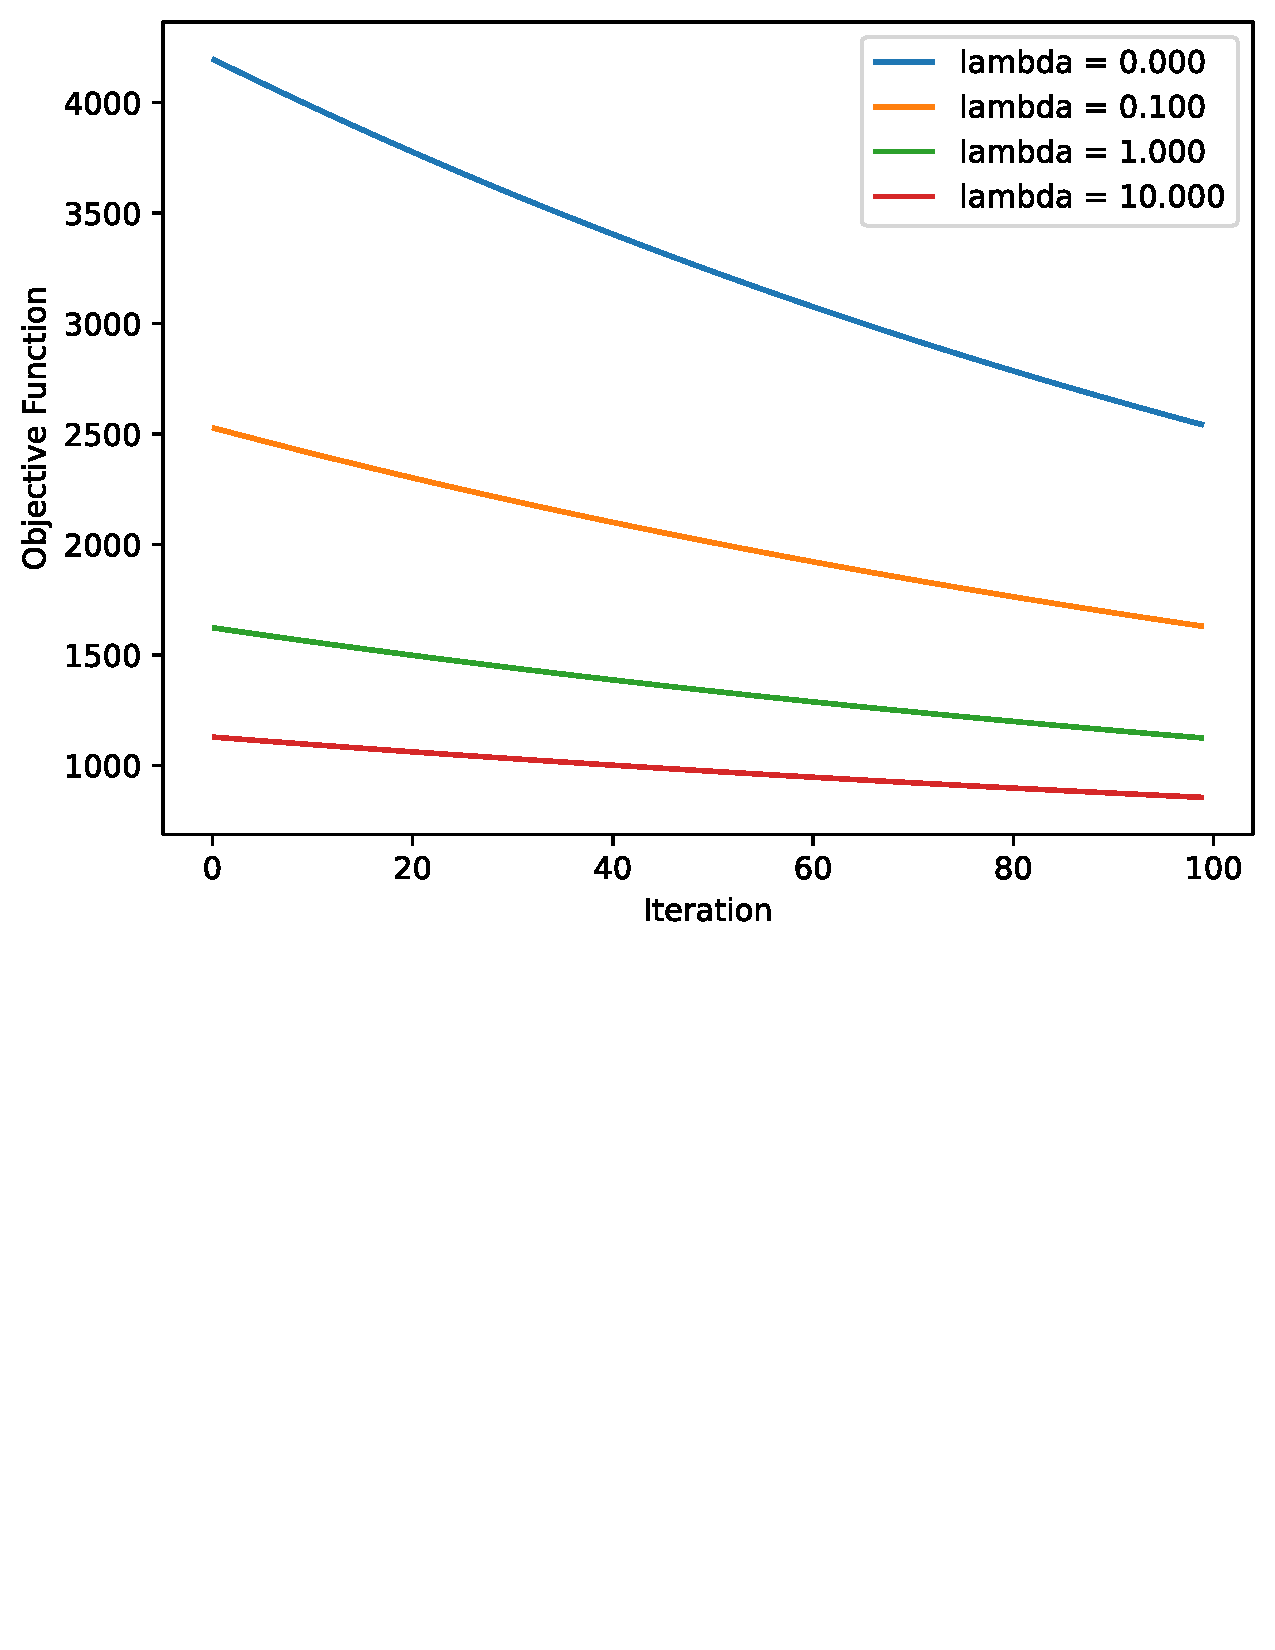
\includegraphics[scale = 0.5]{./6.3.pdf}
        \end{center}
    \end{figure}
\end{sol}
\color{black}
\end{enumerate}
\end{document}

